% Options for packages loaded elsewhere
\PassOptionsToPackage{unicode}{hyperref}
\PassOptionsToPackage{hyphens}{url}
%
\documentclass[
  ngerman,
]{book}
\usepackage{lmodern}
\usepackage{amsmath}
\usepackage{ifxetex,ifluatex}
\ifnum 0\ifxetex 1\fi\ifluatex 1\fi=0 % if pdftex
  \usepackage[T1]{fontenc}
  \usepackage[utf8]{inputenc}
  \usepackage{textcomp} % provide euro and other symbols
  \usepackage{amssymb}
\else % if luatex or xetex
  \usepackage{unicode-math}
  \defaultfontfeatures{Scale=MatchLowercase}
  \defaultfontfeatures[\rmfamily]{Ligatures=TeX,Scale=1}
\fi
% Use upquote if available, for straight quotes in verbatim environments
\IfFileExists{upquote.sty}{\usepackage{upquote}}{}
\IfFileExists{microtype.sty}{% use microtype if available
  \usepackage[]{microtype}
  \UseMicrotypeSet[protrusion]{basicmath} % disable protrusion for tt fonts
}{}
\makeatletter
\@ifundefined{KOMAClassName}{% if non-KOMA class
  \IfFileExists{parskip.sty}{%
    \usepackage{parskip}
  }{% else
    \setlength{\parindent}{0pt}
    \setlength{\parskip}{6pt plus 2pt minus 1pt}}
}{% if KOMA class
  \KOMAoptions{parskip=half}}
\makeatother
\usepackage{xcolor}
\IfFileExists{xurl.sty}{\usepackage{xurl}}{} % add URL line breaks if available
\IfFileExists{bookmark.sty}{\usepackage{bookmark}}{\usepackage{hyperref}}
\hypersetup{
  pdftitle={Wahrscheinlichkeiten},
  pdflang={de},
  hidelinks,
  pdfcreator={LaTeX via pandoc}}
\urlstyle{same} % disable monospaced font for URLs
\usepackage{longtable,booktabs}
\usepackage{calc} % for calculating minipage widths
% Correct order of tables after \paragraph or \subparagraph
\usepackage{etoolbox}
\makeatletter
\patchcmd\longtable{\par}{\if@noskipsec\mbox{}\fi\par}{}{}
\makeatother
% Allow footnotes in longtable head/foot
\IfFileExists{footnotehyper.sty}{\usepackage{footnotehyper}}{\usepackage{footnote}}
\makesavenoteenv{longtable}
\usepackage{graphicx}
\makeatletter
\def\maxwidth{\ifdim\Gin@nat@width>\linewidth\linewidth\else\Gin@nat@width\fi}
\def\maxheight{\ifdim\Gin@nat@height>\textheight\textheight\else\Gin@nat@height\fi}
\makeatother
% Scale images if necessary, so that they will not overflow the page
% margins by default, and it is still possible to overwrite the defaults
% using explicit options in \includegraphics[width, height, ...]{}
\setkeys{Gin}{width=\maxwidth,height=\maxheight,keepaspectratio}
% Set default figure placement to htbp
\makeatletter
\def\fps@figure{htbp}
\makeatother
\setlength{\emergencystretch}{3em} % prevent overfull lines
\providecommand{\tightlist}{%
  \setlength{\itemsep}{0pt}\setlength{\parskip}{0pt}}
\setcounter{secnumdepth}{5}
\usepackage{amsthm}
\usepackage{float}
\usepackage{rotating, graphicx}
\usepackage{multirow}
\usepackage{tabularx}

% new command for pretty oversets with \sim
\newcommand\simcal[1]{\stackrel{\sim}{\smash{\mathcal{#1}}\rule{0pt}{0.5ex}}}

\newcommand{\comma}{,\,}

\floatplacement{figure}{H}

\PassOptionsToPackage{table}{xcolor}

\usepackage{tcolorbox}

\definecolor{kcblue}{HTML}{D7DDEF}
\definecolor{kcdarkblue}{HTML}{2B4E70}

\makeatletter
\def\thm@space@setup{%
  \thm@preskip=8pt plus 2pt minus 4pt
  \thm@postskip=\thm@preskip
}
\makeatother

% \makeatletter % undo the wrong changes made by mathspec
% \let\RequirePackage\original@RequirePackage
% \let\usepackage\RequirePackage
% \makeatother

\newenvironment{rmdknit}
    {\begin{center}
    \begin{tabular}{|p{0.9\textwidth}|}
    \hline\\
    }
    {
    \\\\\hline
    \end{tabular}
    \end{center}
    }

\newenvironment{rmdnote}
    {\begin{center}
    \begin{tabular}{|p{0.9\textwidth}|}
    \hline\\
    }
    {
    \\\\\hline
    \end{tabular}
    \end{center}
    }

\newtcolorbox[auto counter, number within=section]{keyconcepts}[2][]{%
colback=kcblue,colframe=kcdarkblue,fonttitle=\bfseries, title=Key Concept~#2, after title={\newline #1}, beforeafter skip=15pt}

\ifxetex
  % Load polyglossia as late as possible: uses bidi with RTL langages (e.g. Hebrew, Arabic)
  \usepackage{polyglossia}
  \setmainlanguage[]{german}
\else
  \usepackage[shorthands=off,main=ngerman]{babel}
\fi
\ifluatex
  \usepackage{selnolig}  % disable illegal ligatures
\fi
\usepackage[]{natbib}
\bibliographystyle{apalike}

\title{Wahrscheinlichkeiten}
\author{}
\date{\vspace{-2.5em}}

\begin{document}
\maketitle

{
\setcounter{tocdepth}{1}
\tableofcontents
}
\hypertarget{was-erwartet-dich}{%
\chapter*{Was erwartet dich?}\label{was-erwartet-dich}}
\addcontentsline{toc}{chapter}{Was erwartet dich?}

Ein Distanzlernpfad zum Thema \emph{Wahrscheinlichkeiten}

\hypertarget{aktuelles}{%
\subsection*{Aktuelles}\label{aktuelles}}
\addcontentsline{toc}{subsection}{Aktuelles}

\begin{itemize}
\item
  Stichtag für das Kapitel 01 Einführung ist der \textbf{3. März}
\item
  Stichtag für das Kapitel 02 Vorwissen ist der \textbf{8. März}
\end{itemize}

\hypertarget{allgemeine-informationen-zum-ablauf}{%
\subsection*{Allgemeine Informationen zum Ablauf}\label{allgemeine-informationen-zum-ablauf}}
\addcontentsline{toc}{subsection}{Allgemeine Informationen zum Ablauf}

Mit diesem Lernpfad sollst du dir das 4. Kapitel des Schulbuches erarbeiten. Natürlich darfst du das Buch zum Nachlesen und zusätzlichen Üben nutzen. Einige Aufgaben, die hier vorkommen, werden mehr oder weniger aus dem Buch übernommen sein.

Die Arbeit mit einem Lernpfad ist ähnlich der Arbeit mit einem Wochenplan. \textbf{Es gibt Vorgaben, bis wann ein bestimmtes Kapitel oder ein bestimmter Abschnitt durchgearbeitet sein muss.} Und gerade an diesen Stichtagen werden wir vermehrt etwas zusammen durchsprechen. Auch sonst solltest du große Teile deiner Arbeit während der Mathestunden erledigen, da du in diesen ja immer auch die Möglichkeit hast, \textbf{bei Unklarheiten und Verständnisschwierigkeiten nachzufragen.} Natürlich besteht weiterhin die Verpflichtung an den Mathestunden teilzunehmen und \textbf{deine Arbeitsergebnisse am Ende jeder Stunde in OneNote hochzuladen}. Erstelle hierzu bitte immer eine Seite mit dem Tagesdatum als Titel.

Da jede*r von euch über individuelles Vorwissen verfügt, wirst du zum Durcharbeiten dieses Lernpfades nicht genauso lang oder kurz brauchen, wie andere aus deiner Klasse. Es kann sein, dass du auch außerhalb der Mathestunden - also als Hausaufgabe zwischen Mittwoch und Montag - weiterarbeiten musst.

\hypertarget{einfuxfchrung---warum-du-dich-mit-wahrscheinlichkeiten-unbedingt-beschuxe4ftigen-solltest}{%
\chapter{Einführung - Warum du dich mit Wahrscheinlichkeiten unbedingt beschäftigen solltest\ldots{}}\label{einfuxfchrung---warum-du-dich-mit-wahrscheinlichkeiten-unbedingt-beschuxe4ftigen-solltest}}

\href{\%22https://de.wikipedia.org/wiki/Kognitive_Neurowissenschaft\%22}{Kognitive Neurowissenschaftler} bezeichnen das Gehirn gerne als ``Vorhersagemaschine''. Vorhersagen ist demnach allgegenwärtig und wesentliche Funktion des Gehirns. Dabei werden Vorhersagen vor allem dann bewusst, wenn sie nicht eintreffen. Stelle dir zum Beispiel vor, du spielst Tischtennis. Solange der Ball von der Platte wegspringt, wie vorhergesagt, wird dir nicht bewusst, dass du deinen Schläger schon lange, bevor der Ball auf selbigen auftrifft, in Position gebracht hast. Aber wehe auf der Platte liegt ein kleines, unbemerktes Steinchen! Dieses kleine Steinchen macht uns bewusst, dass wir nicht darauf reagieren, wo der Ball ist - das könnten wir gar nicht, die uns bleibende Zeit ist viel zu kurz - , sondern darauf, wohin der Ball unserer Vorhersage zufolge fliegen wird!

So eine Vorhersagemaschine ist für sehr viele Situationen natürlich äußerst praktisch. Sie erleichtert uns den Alltag ungemein. Auch Zukunftsplanungen lassen sich mit ihr machen. Doch wie gut sind wir eigentlich im Vorhersagen?

Bei genauerer Betrachtung müssen wir feststellen, dass wir kaum etwas mit absoluter Sicherheit vorhersagen können. Oft hilft es aber, zumindest über die \textbf{Wahrscheinlichkeit}, mit der ein bestimmtes Ereignis eintritt, gut Bescheid zu wissen. Wie gut wir im Umgang mit solchen Wahrscheinlichkeiten sind, ist also nicht unerheblich! Bedauerlicher Weise müssen wir feststellen, dass wir dabei unter bestimmten Bedingungen recht fehleranfällig zu sein scheinen. Die Psychologie spricht hier auch vom Wahrscheinlichkeitsidioten\ldots.

Wie es um deine Wahrscheinlichkeitseinschätzung bestellt ist, kannst du an den folgenden drei kleinen Aufgaben ausprobieren:

Du bist von den Ergebnissen überrascht? Dann sei gespannt auf mehr.

\hypertarget{vorwissen}{%
\chapter{Vorwissen}\label{vorwissen}}

Wie immer im Matheunterricht baut auch dieses Thema auf bereits gelernten Unterrichtsinhalten auf. Daher findest du hier zunächst eine Checkliste, in der die Voraussetzungen für diesen Lernpfad zusammengestellt sind. Lies sie dir bitte gründlich durch. Solltest du nicht wissen, was mit dem jeweiligen Punkt gemeint ist, oder ahnen, dass du in einem Bereich Lücken hast, bearbeite bitte zunächst die in der letzten Spalte verlinkten Materialien - einfach auf ``nachlesen'' klicken.

Wenn du der Ansicht bist, dass du eigentlich alles (wieder) weißt, geht es mit dem \textbf{Eingangsquiz} weiter. Bearbeite das Quiz und arbeite immer dann, wenn du eine Aufgabe nicht lösen konntest oder sie falsch gelöst hast, die zu diesem Thema auf der Checkliste verlinkten Materialien zum ``Nachlesen'' durch.

\hypertarget{checkliste}{%
\section{Checkliste}\label{checkliste}}

\begin{table}[H]
\centering
\begin{tabular}[t]{l|l|l}
\hline
Themenbereich & Ich kann... & Was war das doch gleich?\\
\hline
Bruchrechnung & ... Brüche kürzen und erweitern. & [nachlesen](https://gdischinger.github.io/W8Extrablatt/BrücheErweiternKürzen.html)\\
\hline
 & ... Brüche als Dezimalzahlen oder in Prozent angeben und umgekehrt. & [nachlesen](https://gdischinger.github.io/W8Extrablatt/DarstellungBruchDeziProzent.html)\\
\hline
 & ... mit Brüchen, Dezimalzahlen und Prozent rechnen. & [nachlesen](https://gdischinger.github.io/W8Extrablatt/Bruchrechnung.html)\\
\hline
deskriptive Statistik & ... absolute und relative Häufigkeiten ermitteln. & nachlesen\\
\hline
 & ... Häufigkeiten in Tabellen, Säulen- und Kreisdiagrammen darstellen. & nachlesen\\
\hline
 & ... das arithmetische Mittel, die Spannweite und den Median angeben. & nachlesen\\
\hline
 & ... Box-Plots interpretieren und erstellen & nachlesen\\
\hline
Wahrscheinlichkeit & ... Zufallsexperimente erkennen und von Vorgängen unterscheiden, die keine Zufallsexperimente sind. & nachlesen\\
\hline
 & ... zu einfachen Zufallsexperimenten die Ergebnismenge erstellen. & nachlesen\\
\hline
 & ... Wahrscheinlichkeiten von Ereignissen angeben. & nachlesen\\
\hline
 & ... die wichtigsten Eigenschaften des mathematischen Wahrscheinlichkeitsbegriffes benennen und anwenden. & nachlesen\\
\hline
 & ... erklären, was das empirische Gesetz der großen Zahlen besagt und ich weiß, wo es seine Anwendung findet. & nachlesen\\
\hline
 & ... Laplace-Experimente erkennen und beschreiben und die zugehörigen Laplace-Wahrscheinlichkeiten angeben. & nachlesen\\
\hline
 & ... erklären, was man unter einer Simulation versteht und einfache Simulationen durchführen. & nachlesen\\
\hline
\end{tabular}
\end{table}

\hypertarget{eingangsquiz}{%
\section{Eingangsquiz}\label{eingangsquiz}}

\hypertarget{mehrstufige-zufallsexperimente}{%
\chapter{Mehrstufige Zufallsexperimente}\label{mehrstufige-zufallsexperimente}}

\hypertarget{baumdiagramme}{%
\chapter{Baumdiagramme}\label{baumdiagramme}}

\hypertarget{ein-baumdiagramm---was-ist-das}{%
\section{Ein Baumdiagramm - Was ist das?}\label{ein-baumdiagramm---was-ist-das}}

\hypertarget{wahrscheinlichkeiten-und-baumdiagramme}{%
\section{Wahrscheinlichkeiten und Baumdiagramme}\label{wahrscheinlichkeiten-und-baumdiagramme}}

\hypertarget{produktregel}{%
\subsection{Produktregel}\label{produktregel}}

\hypertarget{summenregel}{%
\subsection{Summenregel}\label{summenregel}}

\hypertarget{baumdiagramme-geschickt-nutzen}{%
\section{Baumdiagramme geschickt nutzen}\label{baumdiagramme-geschickt-nutzen}}

\hypertarget{uxfcbungsaufgaben}{%
\chapter{Übungsaufgaben}\label{uxfcbungsaufgaben}}

\hypertarget{abschlussquiz}{%
\chapter{Abschlussquiz}\label{abschlussquiz}}

\hypertarget{zusatzmaterial}{%
\chapter*{Zusatzmaterial}\label{zusatzmaterial}}
\addcontentsline{toc}{chapter}{Zusatzmaterial}

\hypertarget{bruchrechnung-kurz-und-knapp}{%
\section*{Bruchrechnung kurz und knapp}\label{bruchrechnung-kurz-und-knapp}}
\addcontentsline{toc}{section}{Bruchrechnung kurz und knapp}

\hypertarget{bruxfcche-kuxfcrzen-und-erweitern}{%
\subsection*{Brüche kürzen und erweitern}\label{bruxfcche-kuxfcrzen-und-erweitern}}
\addcontentsline{toc}{subsection}{Brüche kürzen und erweitern}

Einen Bruch \(a \over b\) mit einer Zahl \(c\) \textbf{erweitern}, bedeutet, dass man \textbf{den Zähler und den Nenner} mit \(c\) \textbf{multipliziert}: \(a \over b\) erweitert mit \(c\) ergibt also \(a \cdot c \over b \cdot c\).

\textbf{Dividiert} man \textbf{Zähler und Nenner} eines Bruches \(x \over y\) durch dieselbe Zahl \(z\), sagt man, \(x \over y\) wird mit \(z\) \textbf{gekürzt}.

Ein Bruch \(e \over f\) heißt \textbf{vollständig gekürzt}, wenn Zähler und Nenner teilerfremd sind. \(2 \over 3\) oder \(1 \over 4\) sind beispielsweise vollständig gekürzt. \(9 \over 15\) dagegen nicht, da man sowohl \(9\) als auch \(15\) durch \(3\) dividieren kann.

\hypertarget{section}{%
\subsubsection*{}\label{section}}
\addcontentsline{toc}{subsubsection}{}

\hypertarget{aufgabe}{%
\subsubsection*{Aufgabe}\label{aufgabe}}
\addcontentsline{toc}{subsubsection}{Aufgabe}

Erweitere \(1 \over 5\) mit \(2\)

\leavevmode\hypertarget{toggleText1}{}%
\(2 \over 10\)

Erweitere \(2 \over 3\) mit \(5\)

\leavevmode\hypertarget{toggleText2}{}%
\(10 \over 15\)

Erweitere \(3 \over 4\) mit \(6\)

\leavevmode\hypertarget{toggleText3}{}%
\(18 \over 24\)

Erweitere \(17 \over 19\) mit \(3\)

\leavevmode\hypertarget{toggleText4}{}%
\(51 \over 57\)

Kürze vollständig: \(8 \over 12\)

\leavevmode\hypertarget{toggleText5}{}%
\(2 \over 3\)

Kürze vollständig: \(8 \over 24\)

\leavevmode\hypertarget{toggleText6}{}%
\(1 \over 3\)

Kürze vollständig: \(72 \over 48\)

\leavevmode\hypertarget{toggleText7}{}%
\(3 \over 2\)

Kürze vollständig: \(21 \over 33\)

\leavevmode\hypertarget{toggleText8}{}%
\(7 \over 11\)

\hypertarget{section-1}{%
\subsubsection*{}\label{section-1}}
\addcontentsline{toc}{subsubsection}{}

\hypertarget{section-2}{%
\subsubsection*{}\label{section-2}}
\addcontentsline{toc}{subsubsection}{}

\hypertarget{bruxfcche-in-dezimalzahlen-oder-prozentangaben-umwandeln}{%
\subsection*{Brüche in Dezimalzahlen oder Prozentangaben umwandeln}\label{bruxfcche-in-dezimalzahlen-oder-prozentangaben-umwandeln}}
\addcontentsline{toc}{subsection}{Brüche in Dezimalzahlen oder Prozentangaben umwandeln}

Möchte man einen Bruch als Dezimalzahl schreiben, muss man den Zähler (schriftlich oder mit Hilfe des Taschenrechners) durch den Nenner dividieren.

Eine Dezimalzahl kann man nun wiederum sehr einfach auch als Prozentzahl angeben: Man verschiebt einfach das Komma um zwei Stellen nach rechts und schreibt hinter die auf diese Weise entstandene Zahl ein \%-Zeichen.

\hypertarget{section-3}{%
\subsubsection*{}\label{section-3}}
\addcontentsline{toc}{subsubsection}{}

\hypertarget{aufgabe-1}{%
\subsubsection*{Aufgabe}\label{aufgabe-1}}
\addcontentsline{toc}{subsubsection}{Aufgabe}

Schreibe als Dezimalzahl\(14 \over 10\)

\leavevmode\hypertarget{toggleText9}{}%
\(1,4\)

Schreibe als Dezimalzahl\(14 \over 100\)

\leavevmode\hypertarget{toggleText10}{}%
\(0,14\)

Schreibe als Dezimalzahl\(12 \over 15\)

\leavevmode\hypertarget{toggleText11}{}%
\(0,8\)

Schreibe als Dezimalzahl\(-{6 \over 4}\)

\leavevmode\hypertarget{toggleText12}{}%
\(-1,5\)

Schreibe in Prozent: \(7 \over 20\)

\leavevmode\hypertarget{toggleText13}{}%
\(35\%\)

Schreibe in Prozent: \(18 \over 48\)

\leavevmode\hypertarget{toggleText14}{}%
\(37,5\%\)

Schreibe in Prozent: \(19 \over 38\)

\leavevmode\hypertarget{toggleText15}{}%
\(50\%\)

Schreibe in Prozent: \(38 \over 19\)

\leavevmode\hypertarget{toggleText16}{}%
\(200\%\)

\hypertarget{section-4}{%
\subsubsection*{}\label{section-4}}
\addcontentsline{toc}{subsubsection}{}

\hypertarget{section-5}{%
\subsubsection*{}\label{section-5}}
\addcontentsline{toc}{subsubsection}{}

\hypertarget{mit-bruxfcchen-rechnen}{%
\subsection*{Mit Brüchen rechnen}\label{mit-bruxfcchen-rechnen}}
\addcontentsline{toc}{subsection}{Mit Brüchen rechnen}

Zwei Brüche werden \textbf{multipliziert}, indem man Zähler mit Zähler und Nenner mit Nenner multipliziert.
\[{a \over b} \cdot {c \over d} = {a \cdot c \over b \cdot d} \]

Durch einen Bruch wird \textbf{dividiert}, indem \textbf{mit seinem Kehrbruch multipliziert} wird.
\[{e \over f} : {x \over y} = {e \cdot y \over f \cdot x}\]

Sollen zwei Brüche \textbf{addiert} oder \textbf{subtrahiert} werden, muss man sie zunächst \textbf{auf den gleichen Nenner bringen}. Anschließend \textbf{addiert} bzw. \textbf{subtrahiert} man die Zähler.

\[{m \over n}+{p \over q} = \frac{m \cdot q}{n \cdot q} + \frac{p \cdot n}{q \cdot n} = {m \cdot q + n \cdot p \over n \cdot q}\]
\[{m \over n}-{p \over q} = \frac{m \cdot q}{n \cdot q} - \frac{p \cdot n}{q \cdot n} = {m \cdot q - n \cdot p \over n \cdot q}\]

\hypertarget{section-6}{%
\subsubsection*{}\label{section-6}}
\addcontentsline{toc}{subsubsection}{}

\hypertarget{aufgabe-2}{%
\subsubsection*{Aufgabe}\label{aufgabe-2}}
\addcontentsline{toc}{subsubsection}{Aufgabe}

\({1 \over 3}\cdot{2 \over 7}\)

\leavevmode\hypertarget{toggleText17}{}%
\(2 \over 21\)

\(-{2 \over 5}\cdot{3 \over 4}\)

\leavevmode\hypertarget{toggleText18}{}%
\(-{3 \over 10}\)

\(7\cdot{6 \over 49}\)

\leavevmode\hypertarget{toggleText19}{}%
\(6 \over 7\)

\({3 \over 4}:{9 \over 10}\)

\leavevmode\hypertarget{toggleText20}{}%
\(5 \over 6\)

\({8 \over 9}:2\)

\leavevmode\hypertarget{toggleText21}{}%
\(4 \over 9\)

\(-{15 \over 14}:(-{10 \over 21})\)

\leavevmode\hypertarget{toggleText22}{}%
\(9 \over 4\)

\({5 \over 6}+{1 \over 4}\)

\leavevmode\hypertarget{toggleText23}{}%
\(13 \over 12\)

\({5 \over 6}-{1 \over 4}\)

\leavevmode\hypertarget{toggleText24}{}%
\(7 \over 12\)

\({12 \over 5}+3\)

\leavevmode\hypertarget{toggleText25}{}%
\(27 \over 5\)

\({2 \over 15}-{11 \over 6}\)

\leavevmode\hypertarget{toggleText26}{}%
\(-{\frac{17}{10}}\)

\({7 \over 3}+{3 \over 2}\)

\leavevmode\hypertarget{toggleText27}{}%
\(23 \over 6\)

\(4-{49 \over 64}\)

\leavevmode\hypertarget{toggleText28}{}%
\(207 \over 64\)

\hypertarget{deskriptive-statistik-zum-nachlesen}{%
\section*{Deskriptive Statistik zum Nachlesen}\label{deskriptive-statistik-zum-nachlesen}}
\addcontentsline{toc}{section}{Deskriptive Statistik zum Nachlesen}

Hätten wir die letzten Monate Präsenzunterricht machen dürfen, hätten wir eine Klassenarbeit über das letzte Thema geschrieben. Schön wäre das gewesen, dann hätten wir jetzt ein Häkchen machen können und gut gelaunt die ersten Frühlingstage verbracht.

Frau D. säße jetzt zuhause in ihrer Küche und würde all die Arbeiten korrigieren. Jedes Mal wenn sie mit einer Arbeit fertig wäre, würde sie die Note auf den dafür vorgesehenen Schmierzettel schreiben. So sähe dieser Schmierzettel dann vielleicht aus:

Noten

Einen solchen Schmierzettel bezeichnet man in der Statistik als \textbf{Urliste}. Auf ihr werden die Ergebnisse einer statistischen Erhebung in der Reihenfolge fesgehalten, in der sie eben auftreten. Daher ist eine \textbf{Urliste} in der Regel unsortiert.

Ordnet man nun die auf der Urliste festgehaltenen Ergebnisse der Größe nach, erhält man eine \textbf{Rangliste}. Wollte Frau D. diese erstellen, sähe sie für das obige Beispiel so aus:

Noten

Aber auch diese - schon etwas ordentlichere - Liste würde euch Frau D. nicht als Ergebnisspiegel präsentieren. Hier hat sich die \textbf{Häufigkeitsliste} durchgesetzt. Auf ihr gibt man zu jedem der möglichen Werte an, wie oft er vorkommt.

Und da sind wir schon bei zwei für dieses Kapitel zentralen Begriffen\ldots{}

\hypertarget{absolute-und-relative-huxe4ufigkeiten-ermitteln}{%
\subsection*{Absolute und relative Häufigkeiten ermitteln}\label{absolute-und-relative-huxe4ufigkeiten-ermitteln}}
\addcontentsline{toc}{subsection}{Absolute und relative Häufigkeiten ermitteln}

Die Anzahl, mit der ein Wert in der erhobenen Urliste vorkommt, heißt \textbf{absolute Häufigkeit} des Wertes. Der Anteil, den die absolute Häufigkeit an der Gesamtzahl der erhobenen Daten hat, heißt \textbf{relative Häufigkeit}.

Zwischen der \textbf{absoluten} und der \textbf{relativen} Häufigkeit besteht also der folgende Zusammenhang:

\[relative \; Häufigkeit = \frac{absolute \; Häufigkeit}{Gesamtzahl\; der\; erhobenen\; Daten}\]

An unserem Notenbeispiel kann man sich das gut verdeutlichen:

Noten

Die \textbf{absolute Häufigkeit} der Note Eins etwa ist \(2\). Die \textbf{absolute Häufigkeit} der Note Vier dagegen ist \(7\).

Wenn ich mich nicht verzählt habe, haben \(22\) Schüler:innen an der Klasenarbeit teilgenommen. Damit erhält man für die Note Eins eine \textbf{relative Häufigkeit} von \(\frac{2}{22} = \frac{1}{11}\) und für die Note Vier eine \textbf{relative Häufigkeit} von \(\frac{7}{22}\).

\hypertarget{section-7}{%
\subsubsection*{}\label{section-7}}
\addcontentsline{toc}{subsubsection}{}

\hypertarget{aufgabe-1-1}{%
\subsubsection*{Aufgabe 1}\label{aufgabe-1-1}}
\addcontentsline{toc}{subsubsection}{Aufgabe 1}

Frau D. hat eine Klassenarbeit korrigiert, an der 26 Schüler:innen teilgenommen haben. Sie hatte auch bereits eine \textbf{Häufigkeitstabelle} erstellt, um eine Übersicht über die Ergebnisse zu erhalten. Leider hat eins ihrer Kinder ein Glas Wasser darüber gekippt. Nun kann man die Hälfte nicht mehr lesen\ldots{}

\begin{longtable}[]{@{}lllllll@{}}
\toprule
Note & 1 & 2 & 3 & 4 & 5 & 6\tabularnewline
\midrule
\endhead
absolute Häufigkeit & 2 & ??? & 10 & ??? & ??? & 1\tabularnewline
relative Häufigkeit & ??? & 0,27 & ??? & 0,15 & 0,08 & ???\tabularnewline
\bottomrule
\end{longtable}

Vervollständige die Tabelle. Gib \textbf{relative Häufigkeiten} auf zwei Nachkommastellen genau an und \textbf{absolute Häufigkeiten} als ganze Zahlen.

\hypertarget{section-8}{%
\subsubsection*{}\label{section-8}}
\addcontentsline{toc}{subsubsection}{}

\hypertarget{aufgabe-2-1}{%
\subsubsection*{Aufgabe 2}\label{aufgabe-2-1}}
\addcontentsline{toc}{subsubsection}{Aufgabe 2}

Beim Torwandschießen wurde die Anzahl der Treffer notiert. Wer hat die beste Torquote?

\begin{longtable}[]{@{}lll@{}}
\toprule
& Anzahl der Schüsse & Anzahl der Treffer\tabularnewline
\midrule
\endhead
R. Lewandowski & \(\quad\quad\quad 32\) & \(\quad\quad\quad 17\)\tabularnewline
D. Alaba & \(\quad\quad\quad 53\) & \(\quad\quad\quad 30\)\tabularnewline
L. Sane & \(\quad\quad\quad 16\) & \(\quad\quad\quad 9\)\tabularnewline
Th. Müller & \(\quad\quad\quad 27\) & \(\quad\quad\quad 16\)\tabularnewline
J. Kimmich & \(\quad\quad\quad 52\) & \(\quad\quad\quad 29\)\tabularnewline
\bottomrule
\end{longtable}

Tipp

Als Torquote bezeichnet man das Verhältnis von getroffenen Toren zur Gesamtanzahl der Schüsse. Wenn du also etwa bei fünf Schüssen dreimal das Tor triffst, dann hast du eine Torquote von \(\frac{3}{5}=0,6\).

\hypertarget{section-9}{%
\subsubsection*{}\label{section-9}}
\addcontentsline{toc}{subsubsection}{}

\hypertarget{aufgabe-3}{%
\subsubsection*{Aufgabe 3}\label{aufgabe-3}}
\addcontentsline{toc}{subsubsection}{Aufgabe 3}

Eine Klasse mit 28 Schüler:innen, von denen 16 Mädchen sind, wird nach ihren Vorlieben und Abneigungen befragt. Dabei geben 14 Schüler:innen an, dass Mathe ihr Lieblingsfach sei. Ein erster Blick auf die erhobenen Daten verrät zudem, dass unter den Matheliebhabern 6 Jungen sind.

Entscheide begründet: Ist Mathe nun bei den Mädchen oder bei den Jungen beliebter?

\hypertarget{section-10}{%
\subsubsection*{}\label{section-10}}
\addcontentsline{toc}{subsubsection}{}

\hypertarget{section-11}{%
\subsubsection*{}\label{section-11}}
\addcontentsline{toc}{subsubsection}{}

\hypertarget{huxe4ufigkeiten-in-tabellen-suxe4ulen--und-kreisdiagrammen-darstellen}{%
\subsection*{Häufigkeiten in Tabellen, Säulen- und Kreisdiagrammen darstellen}\label{huxe4ufigkeiten-in-tabellen-suxe4ulen--und-kreisdiagrammen-darstellen}}
\addcontentsline{toc}{subsection}{Häufigkeiten in Tabellen, Säulen- und Kreisdiagrammen darstellen}

Mit Tabellen und Diagrammen kann man erfasste Werte veranschaulichen. Neben Tabellen hast du sicherlich mindestens \textbf{Säulen-} und \textbf{Kreisdiagramme} kennengelernt.

In \textbf{Säulendiagrammen} kann man die \textbf{absoluten Häufigkeiten} der Werte ablesen. \textbf{Kreisdiagramme} verdeutlichen dagegen den \textbf{Anteil} den ein Wert an der Gesamtheit hat.

Du erinnerst dich, dass Frau D. die Noten, die sie mit ihrer ausgefallenen Klassenarbeit erhoben hat auf einer \textbf{Urliste} notiert hat.

Noten

Um die Mathelage besser einschätzen zu können, greift Frau D. nun in die Trickkiste der deskriptiven (das heißt beschreibenden) Statistik:

Zunächst bringt sie Ordnung ins Chaos, indem sie die Daten tabellarisch darstellt.

\begin{tabular}[t]{l|r|r|r|r|r|r}
\hline
  & 1 & 2 & 3 & 4 & 5 & 6\\
\hline
Anzahl & 2 & 4 & 5 & 7 & 3 & 1\\
\hline
\end{tabular}

Um einen besseren Eindruck von der Verteilung der Daten zu bekommen, fertigt sie nun ein \textbf{Säulendiagramm} an.

\begin{center}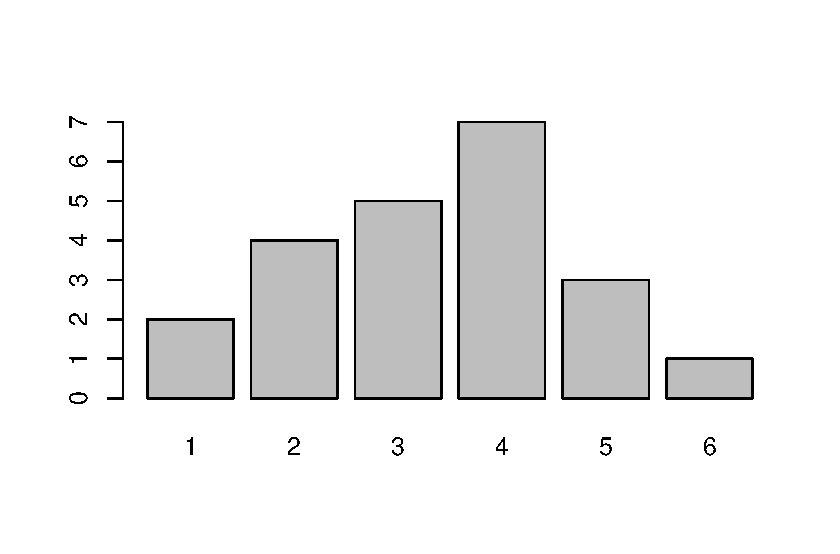
\includegraphics[width=0.9\linewidth]{Wahrscheinlichkeit-8_files/figure-latex/unnamed-chunk-26-1} \end{center}

Schließlich lässt sie sich von ihrem Rechner noch ein \textbf{Kreisdiagramm} erstellen, um eine bildlichere Vorstellung von der relativen Häufigkeit der Noten zu bekommen.

Beim Kreisdiagramm werden Anteile durch passende Winkel am Mittelpunkt des Kreises dargestellt. Der Vollkreis hat 360°. Einer relativen Häufigkeit von \(1\%\) entspricht also ein Kreissektor mit einem Mittelpunktswinkel von \(360° \cdot {1 \over 100} = 3,6°\). Einer relativen Häufigkeit von \(30\%\) entspricht damit ein Kreissektor mit einem Mittelpunktswinkel von \(30 \cdot 3,6° = 108°\)

\begin{center}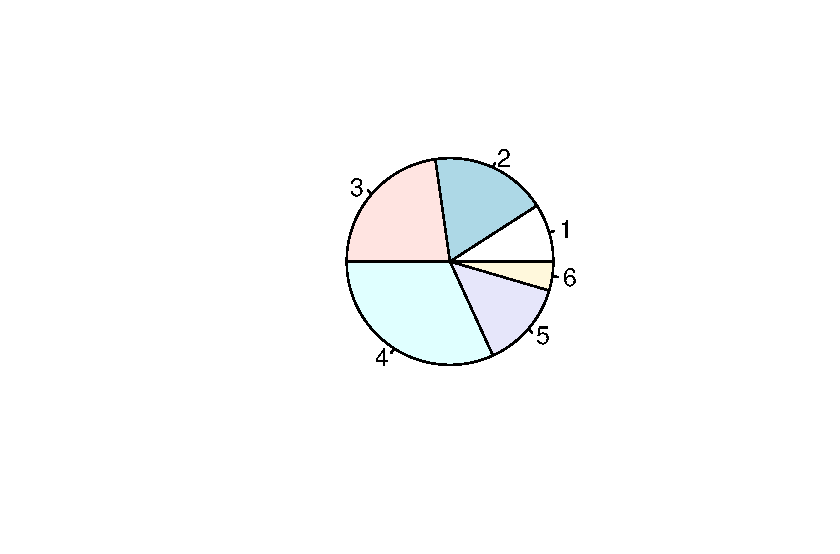
\includegraphics[width=0.9\linewidth]{Wahrscheinlichkeit-8_files/figure-latex/unnamed-chunk-27-1} \end{center}

\hypertarget{section-12}{%
\subsubsection*{}\label{section-12}}
\addcontentsline{toc}{subsubsection}{}

\hypertarget{aufgabe-1-2}{%
\subsubsection*{Aufgabe 1}\label{aufgabe-1-2}}
\addcontentsline{toc}{subsubsection}{Aufgabe 1}

In einer Mathearbeit gab es folgende Noten:

Noten

Erstelle ein Säulen- und ein Kreisdiagramm für die Verteilung der Noten. Du kannst diese Aufgabe per Hand oder mit dem Computer lösen.

Tipp

Für das Kreisdiagramm musst du die relativen Häufigkeiten berechnen.

\hypertarget{section-13}{%
\subsubsection*{}\label{section-13}}
\addcontentsline{toc}{subsubsection}{}

\hypertarget{aufgabe-2-2}{%
\subsubsection*{Aufgabe 2}\label{aufgabe-2-2}}
\addcontentsline{toc}{subsubsection}{Aufgabe 2}

Bei einer Umfrage unter echten Kerlen ergab sich, dass sich \(80\%\) für Fußball interessieren, \(10\%\) gerne Motorrad fahren, \(10\%\) schnelle Autos lieben, sich \(5\%\) für Fußball und schnelle Autos interessieren und \(3\%\) Fussball und ihr Motorrad lieben.

Die Aufgabe lautet: Stelle diesen Sachvervhalt in einem Kreisdiagramm dar.

Anton zeichnet sofort los. Doch schon nach den ersten drei Angaben ist der Kreis ``voll''. Er jammert. Seine kleine Schwester sieht sich seinen Kreis an. Ziemlich schnell hat sie entdeckt, wie man das Problem lösen kann. Dazu muss sie nicht einmal einen neuen Kreis zeichnen.

Was tut sie?

\hypertarget{section-14}{%
\subsubsection*{}\label{section-14}}
\addcontentsline{toc}{subsubsection}{}

\hypertarget{section-15}{%
\subsubsection*{}\label{section-15}}
\addcontentsline{toc}{subsubsection}{}

\hypertarget{das-arithmetische-mittel-die-spannweite-und-den-median-angeben}{%
\subsection*{Das arithmetische Mittel, die Spannweite und den Median angeben}\label{das-arithmetische-mittel-die-spannweite-und-den-median-angeben}}
\addcontentsline{toc}{subsection}{Das arithmetische Mittel, die Spannweite und den Median angeben}

Um kurze und prägnante (oft auch zu kurze!) Aussagen mit Hilfe der erhobenen Daten treffen zu können, bedient man sich der statistischen \textbf{Kennwerte}. Auch von diesen kennst du schon einige.

Das \textbf{arithmetische Mittel} beispielsweise ist Bestandteil des Alltags: Wenn wir vom ``Durchschnitt'' sprechen, meinen wir meist arithmetische Mittelwerte. Du erwartest ihn vermutlich auch als Angabe unter einer Klassenarbeit.

Das \textbf{arithmetische Mittel} berechnet man als \textbf{die Summe aller Werte durch die Anzahl der Werte}. Sehen wir uns als Beispiel die Fehleranzahl von 5 Grundschüler:innen in einem Diktat an.

\begin{longtable}[]{@{}ll@{}}
\toprule
& Anzahl der Fehler\tabularnewline
\midrule
\endhead
Anna & \(\quad\quad\quad 0\)\tabularnewline
Barbara & \(\quad\quad\quad 2\)\tabularnewline
Claire & \(\quad\quad\quad 4\)\tabularnewline
Dennis & \(\quad\quad\quad 3\)\tabularnewline
Enno & \(\quad\quad\quad 5\)\tabularnewline
\bottomrule
\end{longtable}

Das \textbf{arithmetische Mittel} ergibt sich also hier wie folgt:
\[\bar{x} = \frac{0+2+4+3+5}{5} = \frac{14}{5} =2,8\]

Das \textbf{arithmetische Mittel} hat allerdings einen kleinen Schwachpunkt. Es lässt sich - wie man sagt - von Ausreißern beeinflussen. Was das heißt, erkennt man ganz gut in dem Fall, in dem der arme Enno nicht ein einziges Wort richtig geschrieben hat\ldots{}

\begin{longtable}[]{@{}ll@{}}
\toprule
& Anzahl der Fehler\tabularnewline
\midrule
\endhead
Anna & \(\quad\quad\quad 0\)\tabularnewline
Barbara & \(\quad\quad\quad 2\)\tabularnewline
Claire & \(\quad\quad\quad 4\)\tabularnewline
Dennis & \(\quad\quad\quad 3\)\tabularnewline
Enno & \(\quad\quad\quad 131\)\tabularnewline
\bottomrule
\end{longtable}

Wenn der Grundschullehrer nun in einer Konferenz besorgt mitteilen würde, dass die Kinder im Diktat im Durchschnitt 28 Fehler machen, wäre dies sicher keine angemessene Aussage über die tatsächliche Leistung der Schüler:innen. Während Anna, Barbara, Claire und Dennis viel zu schlecht dastünden, käme Enno wiederum viel zu gut weg.

Diesen Nachteil hat der \textbf{Median} nicht (er hat andere :) )

\hypertarget{box-plots-interpretieren-und-erstellen}{%
\subsection*{Box-Plots interpretieren und erstellen}\label{box-plots-interpretieren-und-erstellen}}
\addcontentsline{toc}{subsection}{Box-Plots interpretieren und erstellen}

\begin{tabular}[t]{l|r|r|r|r|r|r}
\hline
  & 1 & 2 & 3 & 4 & 5 & 6\\
\hline
Anzahl & 18 & 0 & 0 & 0 & 0 & 12\\
\hline
\end{tabular}

\begin{center}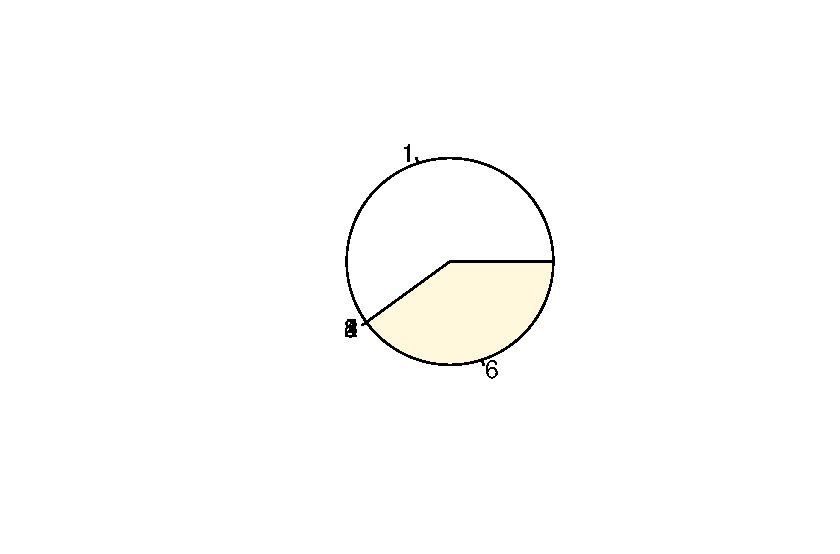
\includegraphics[width=0.9\linewidth]{Wahrscheinlichkeit-8_files/figure-latex/unnamed-chunk-32-1} \end{center}

\begin{center}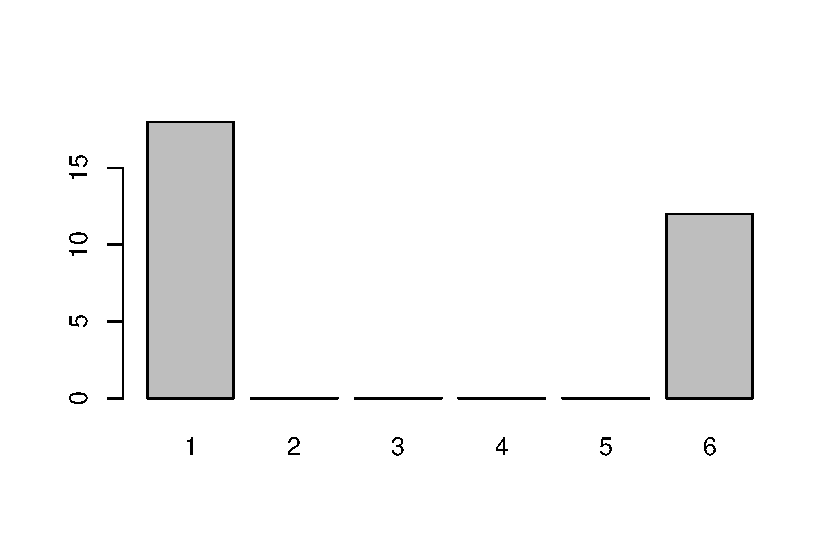
\includegraphics[width=0.9\linewidth]{Wahrscheinlichkeit-8_files/figure-latex/unnamed-chunk-32-2} \end{center}

\begin{center}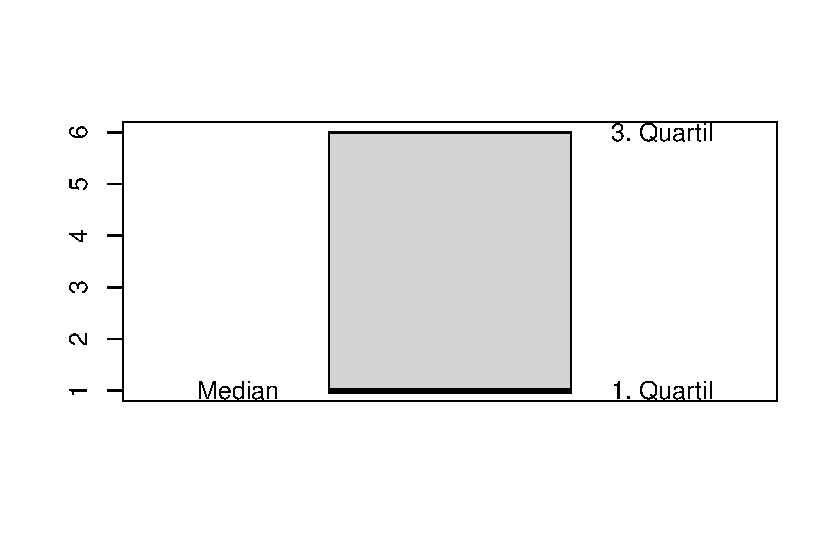
\includegraphics[width=0.9\linewidth]{Wahrscheinlichkeit-8_files/figure-latex/unnamed-chunk-32-3} \end{center}

\hypertarget{wahrscheinlichkeit---da-war-doch-was}{%
\section*{Wahrscheinlichkeit - da war doch was}\label{wahrscheinlichkeit---da-war-doch-was}}
\addcontentsline{toc}{section}{Wahrscheinlichkeit - da war doch was}

\hypertarget{zufallsexperimente-erkennen}{%
\subsection*{Zufallsexperimente erkennen}\label{zufallsexperimente-erkennen}}
\addcontentsline{toc}{subsection}{Zufallsexperimente erkennen}

\hypertarget{die-ergebnismenge-eines-einfachen-zufallsexperiments}{%
\subsection*{Die Ergebnismenge eines einfachen Zufallsexperiments}\label{die-ergebnismenge-eines-einfachen-zufallsexperiments}}
\addcontentsline{toc}{subsection}{Die Ergebnismenge eines einfachen Zufallsexperiments}

\hypertarget{die-wahrscheinlichkeit-eines-ereignisses}{%
\subsection*{Die Wahrscheinlichkeit eines Ereignisses}\label{die-wahrscheinlichkeit-eines-ereignisses}}
\addcontentsline{toc}{subsection}{Die Wahrscheinlichkeit eines Ereignisses}

\hypertarget{der-mathematische-wahrscheinlichkeitsbegriff}{%
\subsection*{Der mathematische Wahrscheinlichkeitsbegriff}\label{der-mathematische-wahrscheinlichkeitsbegriff}}
\addcontentsline{toc}{subsection}{Der mathematische Wahrscheinlichkeitsbegriff}

\hypertarget{das-empirische-gesetz-der-grouxdfen-zahlen}{%
\subsection*{Das empirische Gesetz der großen Zahlen}\label{das-empirische-gesetz-der-grouxdfen-zahlen}}
\addcontentsline{toc}{subsection}{Das empirische Gesetz der großen Zahlen}

\hypertarget{laplace-experimente-und-ihre-wahrscheinlichkeiten}{%
\subsection*{Laplace-Experimente und ihre Wahrscheinlichkeiten}\label{laplace-experimente-und-ihre-wahrscheinlichkeiten}}
\addcontentsline{toc}{subsection}{Laplace-Experimente und ihre Wahrscheinlichkeiten}

\hypertarget{simulationen}{%
\subsection*{Simulationen}\label{simulationen}}
\addcontentsline{toc}{subsection}{Simulationen}

  \bibliography{book.bib,packages.bib}

\end{document}
